\subsection{Factors influencing the shape of the peaks}\label{factorshape}
Before discussing the procedures of measuring the shape of the absorption peaks, it was necessary to analyse which factors had influence on this shape in all the measurements we did. The most important ones were mode hopping, multimodal emission and low-pass deformation, which are discussed in the subsequent paragraphs. Other factors such as
\begin{itemize}
\item variations in the speed of the chopper
\item variations in the oxygen pressure and concentration
\item sample rate of our instruments
\item cable capacitance 
\end{itemize}
should have been not relevant when compared to the first three factors.

\subsubsection{Mode hopping} 
Mode hopping is the factor which most distorted the shape of the measured peaks, limiting us to see only a portion of them. As discussed in \cref{tuna}, the linear range of tunability we can exploit to scan the absorption peak is indeed smaller than the peak width. As the laser exits this interval, a mode jump happens, thus making the photoacoustic resonance to fade away. We got around this by logging the wavelength of the emission peak, measured with the spectrometer and calculated by the \textit{Avaspec}\textsuperscript{\copyright} software in real time\footnote{within a response time less than 10$^{-1}$ s.}. Superimposing this data to the acoustic magnitude ones we could distinguish between the parts of the peaks which really corresponded to the absorption peak shape and the parts affected by mode-hopping.

\subsubsection{Multimodes}
The ECDL didn't always emit light on a single wavelength, but often it would emit in 2 or 3, rarely on 4, different wavelengths at the same time. One or more of these emissions could correspond to one of the oxygen absorption lines, thus generating a measurable photoacoustic effect (\cref{multimodes}). This situation rose the problem that the relative intensity of the various emitted wavelengths was not constant even within the tunability range. Therefore the shape of the peak in such situation could be distorted by the change of intensity. In addition, our apparatus could log and register only the wavelength and intensity of the strongest emitted peak, even when the laser was not emitting in a single mode. This made very difficult to distinguish between single-mode and multi-mode emissions just looking at the recorded data. 
Indeed the only way we had to suppose a multi-modal emission according to the recorded data was looking for
\begin{itemize}
\item fast jumps between two wavelengths competing in being the main one
\item decreases in the main peak intensity or in the intensity-peak integral ratio, though difficult because these two parameters were quite noisy.
\end{itemize}
The best solution we found, however, was to personally attend to the measurements and observe the etalon interference pattern to detect multi-modal emissions. Also it was important to try many different sets of laser parameters, in order to avoid multimodal emissions which contained absorption wavelengths.

\begin{figure}
\includegraphics[width=\linewidth, draft=\foto]{eps/multimode.eps}
\caption{We can see two different absorption peaks, both of them appearing during a multimodal laser emission. The first peak corresponds to a wavelength of 687.40 nm but suddenly jumps to a wavelength of 686.65 nm, while the second corresponds to an absorption wavelength of 687.30 nm but jumps back and forth several times between to the frequency of 687.05 nm. This means that the laser is emitting in at least two different modes at the same time and while initially one of the two is the strongest, after a bit the other becomes higher and the spectrometer starts indicating it as the main peak. In such a situation the shape of the peak is severely deformed by the changes in intensity of the various modes.
Laser parameters: 29.10\cel; 73.23 mA.}
\label{multimodes}
\end{figure} 

\subsubsection{Noise and lock-in low pass filter}
The lock-in amplifier we used contained an adjustable low pass filter to control the output signals. A higher time constant allows to filter out more noise, but on the other side it would correspond to a lower slew rate of the signal. This deformed the shape of the peaks, especially when the signal changed abruptly during a mode hop or in fast sweep measurement. After several attempts we found that a time constant of 1 second gave a quite stable output without requiring us to make too slow measurements.